\section{Photon Conversion Reconstruction}
\label{standard}


Up to 70\% of photons traversing the Tracker material converts into  $e^+ e^-$ pairs.
In the Minimum Bias events collected during the  first phase of CMS data taking, photons, mainly coming from
$\pi^0$ decays, are expected to have a very soft spectrum. The electron pairs from conversions are very unlikely to
reach the Electromagnetic Calorimeter (ECAL) and the ECAL cluster-driven track and seed finding method~\cite{NOTE2006005, EGM-10-005}
cannot be applied. The development of the iterative tracking described in~\cite{TRK-10-001}
largely extended the capability of reconstructing low-\pt tracks and displaced vertices.
Furthermore, for the work presented in this Analysis Summary, additional seeding steps were introduced as described in Sec.~\ref{sec:newSeedingSteps}
and exploited here to improve the identification of conversions at large radii.
The tracker-only conversion reconstruction was already partially commissioned with limited statistics
during the LHC runs at $\sqrt{s}=900\GeV$ data~\cite{TRK-10-001}.


The conversion information can be obtained by the reconstruction of the e+ and e? tracks of the
	conversion. Two methods are used and compared, ECAL-seeded conversion method and combined conversion method. One method only uses the conversion ECAL-seeded tracks and the 	other takes into account conversion track pairs reconstructed from a combination of standard 	tracks, Gaussian sum filter (Gsf) tracks and conversion ECAL-seeded tracks. We first check various kinematical distributions of selected photons in ECAL-seeded conversion method, followed by combined conversion method.


Both methods (ECAL-seeded and combined) 	fit two oppositely charged tracks to a common vertex with the constraint that the two tracks 	are parallel at the vertex, in both the transverse and longitudinal planes. The methods differ 	mainly in the preselection of the track pairs.

%\subsection{Selection and results}                                                                                                                                                                


Photon conversions are characterized by a pair of
oppositely charged secondary tracks, originating from the photon vertex with an
invariant mass consistent with zero,  which are therefore parallel
to each other at production vertex. The electron-positron pair, then,
opens only in the transverse plane because of the solenoidal magnetic field.



In this analysis we use the tracker-driven conversion reconstruction,
already described in~\cite{TRK-10-001}, in~\cite{trk10001} and in~\cite{TRK-10-003}. We
summarize the method here mentioning the further requirements needed to  
specialize the tracker conversion reconstruction to the $\chi_c$
case. The algorithm relies on the capability of iterative tracking,
discussed in~\cite{TRK-10-001}, to efficiently reconstruct low-\pt and
displaced tracks, as the ones coming from a photon conversion.

Opposite-sign track pairs are firstly required to satisfy basic
quality criteria, i.e. have more than four hits and a normalised
$\chi^2$ less than 10. Then
the tracker-only conversion finding exploits the conversion pair
signature to distinguish genuine pairs from fake pairs.
Tracks are required to have positive charge-signed transverse impact
parameter (the primary vertex lies outside the track trajectory helix)
and the distance of minimum approach in the $xy$ plane, $d_m$, between $-0.25\cm$
and $1\cm$ where $d_m$ is
%defined as $d_{O_1-O_2} - (R_1 - R_2)$ where
%$d_{O_1-O_2}$ is the distance between the centres of the two track
%circles in the transverse plane and $R_1$ and $R_2$ are the two
%circles radii.
the distance between the two points of tangent approach in the
transverse plane for the helices of the two tracks.




Track pairs surviving the selection are then fitted to a common
3D-constrained kinematic vertex fitter. The 3D constraints imposes the
tracks to be parallel in both the transverse and longitudinal planes.
The pair is retained if the fit converges and its $\chi^2$ probability
is greater than $5\times10^{-4}$.



Conversion vertices are reconstructed with an excellent precision:
the angular resolution is about $1{\rm mrad}$ while the radial resolution varies from about~$0.2\cm$ to about~$0.5\cm$, primarily
as a function of pseudo-rapidity.
In Fig.~\ref{fig:convXY} the position of conversion vertices reconstructed in data is shown in the $(x,y)$ plane:
in Fig.~\ref{subfig:convXY_a} the structure at the very centre is the Pixel detector,
surrounded by the shell and rails supporting the Pixel detector, four layers of the Inner Tracker and the first layer of the Outer Tracker.
When restricting the $(x,y)$ view to $\pm 12\cm$, Fig.~\ref{subfig:convXY_c}, the beam pipe is clearly visible, off-centered with respect to
the Pixel detector. More details on the features visible on the ``radiographies'' are given in Sec.~\ref{sec:mat}.

The  $(z, R)$  view of conversion vertices reconstructed in data is finally shown in Fig.~\ref{fig:convRZ};  the less populated
areas  around $|\eta|\sim1.2$, also present in simulation, correspond to transition regions between the Tracker
barrel and endcap sub-components for which the additional track seeding
iterations described in Sec.~\ref{sec:newSeedingSteps} have not been optimized and the conversion reconstruction efficiency is smaller.

\begin{figure}[h!]
  \begin{center}
   \vspace{-0.6cm}
   \subfigure[]{
   \label{subfig:convXY_a}
    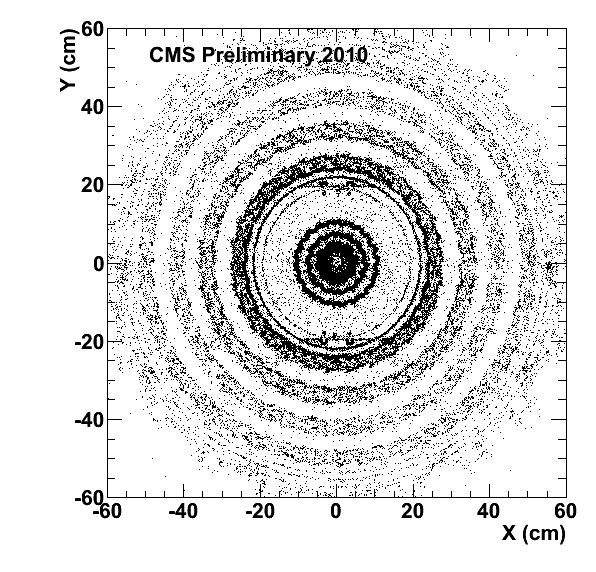
\includegraphics[width=0.40\textwidth]{fig/conversions/ptCut/data_xy.png}}
   \subfigure[]{
   \label{subfig:convXY_b}
    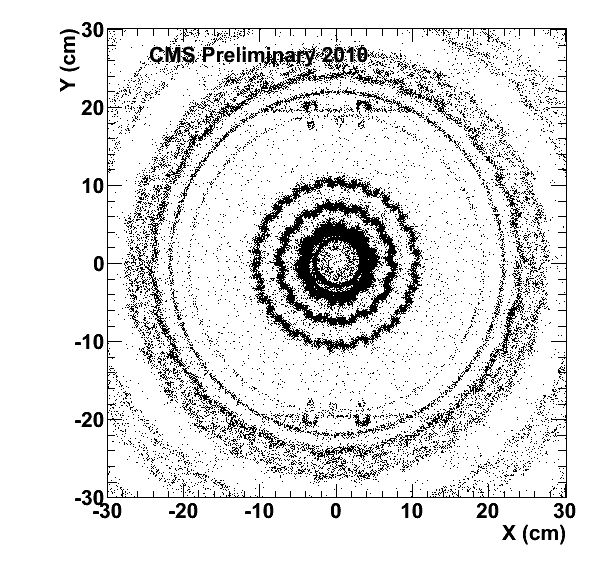
\includegraphics[width=0.40\textwidth]{fig/conversions/ptCut/data_xy_zoom.png}}
   \subfigure[]{
   \label{subfig:convXY_c}
    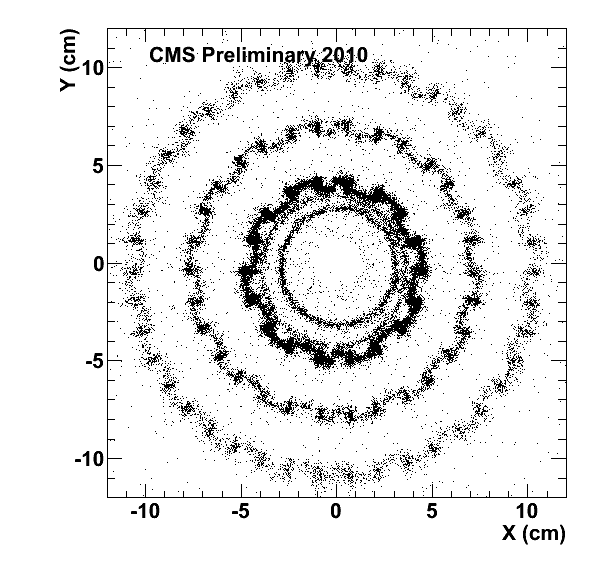
\includegraphics[width=0.40\textwidth]{fig/conversions/ptCut/data_xy_pixel_eta.png}}
    \caption{Conversion vertices in data in the $(x,y)$ plane for $|z|<26\cm$; zoom increases from (a) to (c).}
    \label{fig:convXY}
  \end{center}
\end{figure}

\begin{figure}[h!]
  \begin{center}
     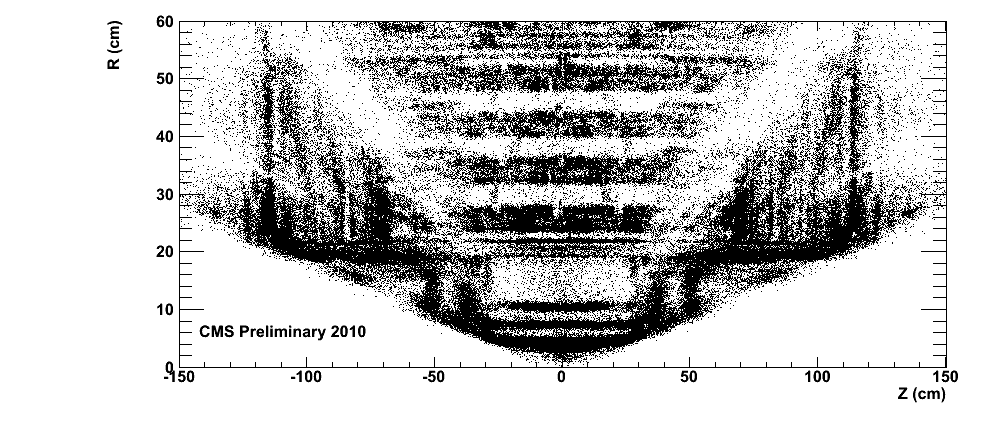
\includegraphics[width=15cm,height=5.5cm]{fig/conversions/ptCut/data_rz.png}
      \caption{Conversion vertices in data the $(z,R)$ plane.}
    \label{fig:convRZ}
  \end{center}
\end{figure}


\begin{figure}[!hbtp]
\centering
\subfigure[]{
\label{subfig:TIBL1Int_LocView_sim}
\includegraphics[width=.32\textwidth]{fig/L1_INT_sim_mod.png}}
\subfigure[]{
\label{subfig:TIBL1Int_LocView_mc}
\includegraphics[width=.32\textwidth]{fig/L1_INT_mc_mod.png}}
\subfigure[]{
\label{subfig:TIBL1Int_LocView_data}
\includegraphics[width=.32\textwidth]{fig/L1_INT_data_mod.png}}
\caption{Nuclear interaction local view of the $x_{\rm local}$ vs. $z_{\rm local}$ projection related to the Inner Tracker Layer 1, internal part: \subref{subfig:TIBL1Int_LocView_sim}~simulation\
 truth; \subref{subfig:TIBL1Int_LocView_mc}~simulation reconstructed; \subref{subfig:TIBL1Int_LocView_data}~data.}
\label{fig:TIBL1Int_LocView}
\end{figure}

As an example of this technique, the local transverse view, $x_{\rm local}$ vs. $z_{\rm local}$ with respect to the R$\phi$ module, of the Inner Strip Tracker Layer 1, internal, is shown in Fig.\
~\ref{fig:TIBL1Int_LocView} for nuclear interaction vertices. Each plot features the single module local view replicated three times, with the appropriate relative geometry, to mock-up a portion\
 of the structure.
The data based plot of Fig.~\ref{fig:TIBL1Int_LocView}~\subref{subfig:TIBL1Int_LocView_data} shows the structures expected in the simulation but affected by the smearing due to misalignment and \
unavoidable irregularities of the passive structures.


